\documentclass[12pt]{article}
\usepackage{setspace}  % To use linespacing
\usepackage{indentfirst} % Indents first line after sections
\usepackage{amssymb} % For \mathbb
\usepackage{enumerate} % For changing labels of enumerate
\usepackage[margin=1in]{geometry} % For editing margins
\usepackage{tikz} % Tikz drawing for graphs
\usetikzlibrary{arrows.meta} % Allows customizing arrows
\usetikzlibrary{backgrounds} % For framing a tikzpicture
\usepackage{amsmath}

% Make new commands
\newcommand{\N}{\mathbb{N}}
\newcommand{\R}{\mathbb{R}}
\newcommand{\Z}{\mathbb{Z}}
\newcommand{\abs}[1]{\left|#1\right|}
\newcommand{\paren}[1]{\left(#1\right)}
\newcommand{\fivespace}{\space\space\space\space\space}

\newcommand{\be}{\begin{enumerate}}
\newcommand{\ee}{\end{enumerate}}
\newcommand{\seti}[1]{\setcounter{enumi}{#1}}
\newcommand{\setii}[1]{\setcounter{enumii}{#1}}

% Start main document
\begin{document}
\onehalfspacing
\hfill Frank Cline

\hfill Math 307

\hfill HW 7

% Sections
% 6.3 # 2, 8, 11a
% 6.4 # 6, 8, 10, 12 and additional problems
% 6.5 # 2, 4, 8
% 4.6 # 8

% SECTION 6.3 # 2, 8, 11a
\section*{6.3}
\be

% 8
\seti{7}
\item Consider a tree with $n$ vertices. It has exactly $n-1$ edges [Lemma 2], so the sum of its of the degrees of its vertices is $2n-2$.
	\be
	% 8a
	\item A tree has two vertices of degree 5, three of degree 3, two of degree 2, and the rest of degree 1. 	How many vertices are in the graph?\\
	$2|E(G)| = 2n-2 = 2(5)+3(3)+2(2)+x$
	
	\ee

% 11a
\seti{10}
\item
	\be
	% 11a
	\item Show that a forest with $n$ vertices and $m$ components has $n-m$ edges.\\
	Suppose the components have $n_1,n_2,n_3,...,n_m$ vertices. The total vertices of the forest is then 
	$n_1+n_2+n_3+...+n_m=n$. The $i$th component is a tree, so it has $n_i-1$ edges by Theorem 4. The total amount of edges in 
	the forest is then $(n_1-1)+(n_2-1)+(n_3-1)+...+(n_m-1)=n-m$.
	\ee
\ee

% SECTION 6.4 % 6, 8, 10, 12, and additional problems
\section*{6.4}
\be

% 6
\seti{5}
\item 
	\be
	% 6a
	\item Draw each of the seven types of rooted trees of height 3 in which each node that is not a leaf has 2 
	children.\\
	% 6a 1
	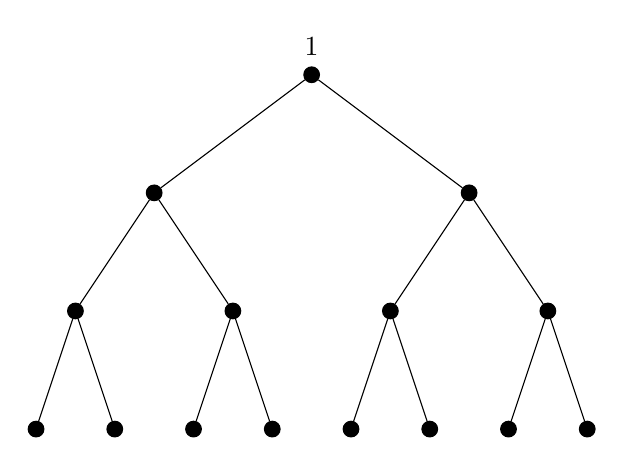
\begin{tikzpicture}[scale = 1,every node/.style={circle,draw, fill= black, inner sep = 2pt},level 1/.style={sibling 				distance=40mm},level 2/.style={sibling distance=20mm},level 3/.style={sibling distance=10mm}]
	
	\node[label = above:1] {}
	child {
		node{} 
		child {node{}
			child {node{}} 
			child {node{}} }			 
		child {node{}
			child {node{}} 
			child {node{}} }
	}
	child {
		node{} 
		child {node{}
			child {node{}} 
			child {node{}} }			 
		child {node{}
			child {node{}} 
			child {node{}} }
	};	
	\end{tikzpicture}

	% 6a 2
	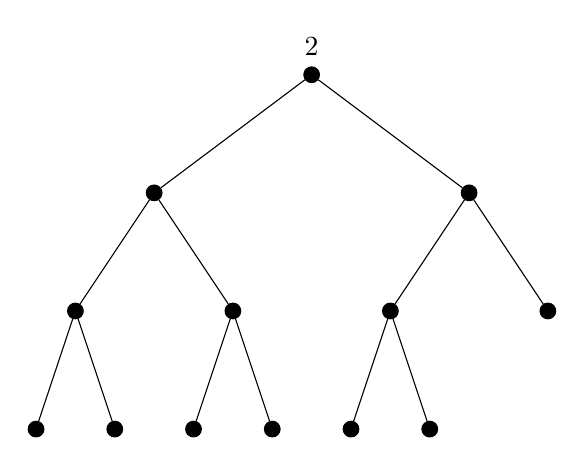
\begin{tikzpicture}[scale = 1,every node/.style={circle,draw, fill= black, inner sep = 2pt},level 1/.style={sibling 				distance=40mm},level 2/.style={sibling distance=20mm},level 3/.style={sibling distance=10mm}]
	
	\node[label = above:2] {}
	child {
		node{} 
		child {
			node{}
			child {
				node{}
			}
			child {
				node{}
			}
		}
		child {
			node{}
			child {
				node{}
			}
			child {
				node{}
			}
		}
	}
	child {
		node{} 
		child {
			node{}
			child {
				node{}
			}
			child {
				node{}
			}
		}
		child {
			node{}
		}
	};	
	\end{tikzpicture}

	% 6a 3
	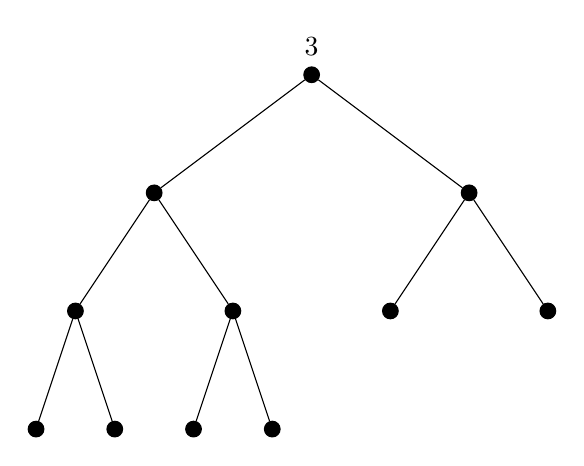
\begin{tikzpicture}[scale = 1,every node/.style={circle,draw, fill= black, inner sep = 2pt},level 1/.style={sibling 				distance=40mm},level 2/.style={sibling distance=20mm},level 3/.style={sibling distance=10mm}]
	
	\node[label = above:3] {}
	child {
		node{} 
		child {
			node{}
			child {
				node{}
			}
			child {
				node{}
			}
		}
		child {
			node{}
			child {
				node{}
			}
			child {
				node{}
			}
		}
	}
	child {
		node{} 
		child {
			node{}
		}
		child {
			node{}
		}
	};	
	\end{tikzpicture}

	% 6a 4
	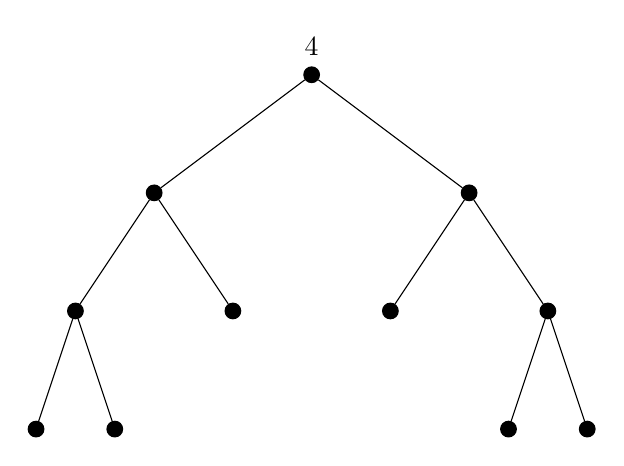
\begin{tikzpicture}[scale = 1,every node/.style={circle,draw, fill= black, inner sep = 2pt},level 1/.style={sibling 				distance=40mm},level 2/.style={sibling distance=20mm},level 3/.style={sibling distance=10mm}]
	
	\node[label = above:4] {}
	child {
		node{} 
		child {
			node{}
			child {
				node{}
			}
			child {
				node{}
			}
		}			
		child {
			node{}
		}
	}
	child {
		node{} 
		child {
			node{}
		}
		child {
			node{}
			child {
				node{}
			}
			child {
				node{}
			}
		}
	};	
	\end{tikzpicture}

	% 6a 5
	\begin{tikzpicture}[scale = 1,every node/.style={circle,draw, fill= black, inner sep = 2pt},level 1/.style={sibling 				distance=40mm},level 2/.style={sibling distance=20mm},level 3/.style={sibling distance=10mm}]
	\node[label = above:5] {}
	child {
		node{} 
		child {
			node{}
			child {
				node{}
			}
			child {
				node{}
			}
		}
		child {
			node{}
		}
	}
	child {
		node{} 
		child {
			node{}
		}
		child {
			node{}
		}
	};	
	\end{tikzpicture}

	% 6a 6
	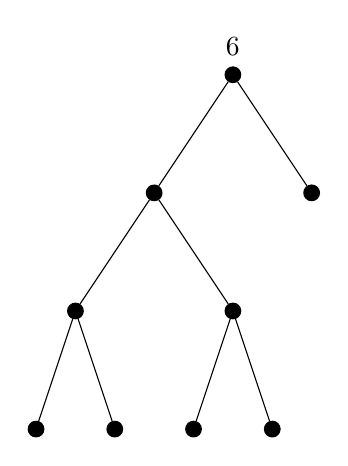
\begin{tikzpicture}[scale = 1,every node/.style={circle,draw, fill= black, inner sep = 2pt},level 1/.style={sibling 				distance=20mm},level 2/.style={sibling distance=20mm},level 3/.style={sibling distance=10mm}]
	\node[label = above:6] {}
	child {
		node{} 
		child {
			node{}
			child {
				node{}
			}
			child {
				node{}
			}
		}
		child {
			node{}
			child {
				node{}
			}
			child {
				node{}
			}
		}
	}
	child {
		node{} 
	};	
	\end{tikzpicture}	

	% 6a 7
	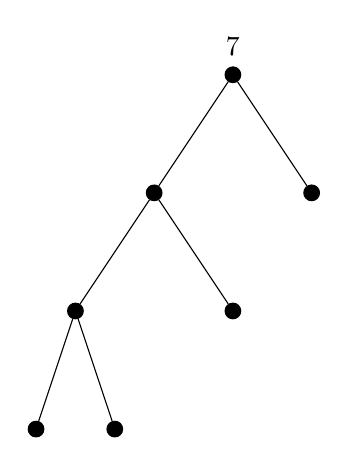
\begin{tikzpicture}[scale = 1,every node/.style={circle,draw, fill= black, inner sep = 2pt},level 1/.style={sibling 				distance=20mm},level 2/.style={sibling distance=20mm},level 3/.style={sibling distance=10mm}]
	\node[label = above:7] {}
	child {
		node{} 
		child {
			node{}
			child {
				node{}
			}
			child {
				node{}
			}
		}
		child {
			node{}
		}
	}
	child {
		node{} 
	};	
	\end{tikzpicture}
	\ee

% 8
\seti{7}
\item A 2-3 tree is a rooted tree such that each interior node, including the root if the height is 2 or more, has either two or three children and all paths from the root to the leaves habe the same length. There are seven different types of 2-3 trees of height 2. Draw one tree of each type.\\
	% 8 - 1
	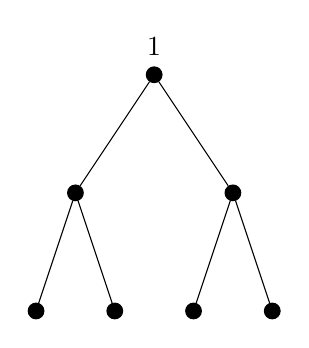
\begin{tikzpicture}[scale = 1,every node/.style={circle,draw, fill= black, inner sep = 2pt},level 1/.style={sibling 				distance=20mm},level 2/.style={sibling distance=10mm}]
	
	\node[label = above:1] {}
	child {
		node{} 
		child {
			node{}
		}			
		child {
			node{}
		}
	}
	child {
		node{} 
		child {
			node{}
		}
		child {
			node{}
		}
	};	
	\end{tikzpicture}

	% 8 - 2
	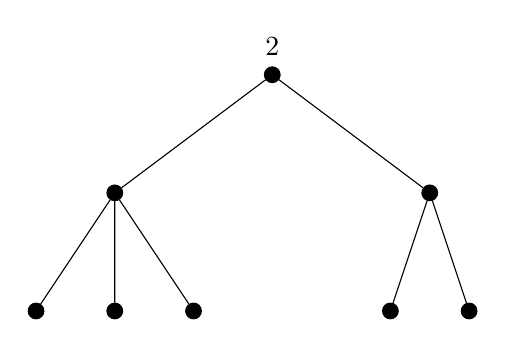
\begin{tikzpicture}[scale = 1,every node/.style={circle,draw, fill= black, inner sep = 2pt},level 1/.style={sibling 				distance=40mm},level 2/.style={sibling distance=10mm}]
	
	\node[label = above:2] {}
	child {
		node{} 
		child {
			node{}
		}			
		child {
			node{}
		}
		child {
			node{}
		}
	}
	child {
		node{} 
		child {
			node{}
		}			
		child {
			node{}
		}
	};	
	\end{tikzpicture}


	% 8 - 3
	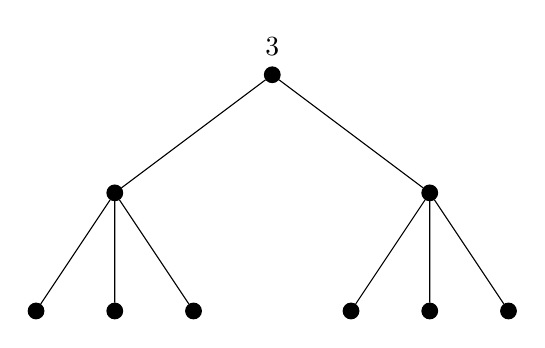
\begin{tikzpicture}[scale = 1,every node/.style={circle,draw, fill= black, inner sep = 2pt},level 1/.style={sibling 				distance=40mm},level 2/.style={sibling distance=10mm}]
	
	\node[label = above:3] {}
	child {
		node{} 
		child {
			node{}
		}			
		child {
			node{}
		}
		child {
			node{}
		}
	}
	child {
		node{} 
		child {
			node{}
		}			
		child {
			node{}
		}
		child {
			node{}
		}
	};	
	\end{tikzpicture}

	% 8 - 4
	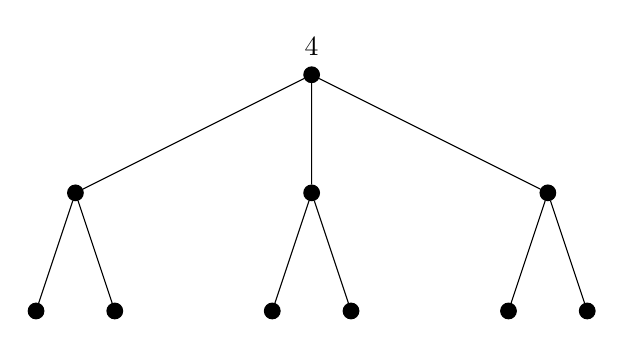
\begin{tikzpicture}[scale = 1,every node/.style={circle,draw, fill= black, inner sep = 2pt},level 1/.style={sibling 				distance=30mm},level 2/.style={sibling distance=10mm}]
	
	\node[label = above:4] {}
	child {
		node{} 
		child {
			node{}
		}			
		child {
			node{}
		}
	}
	child {
		node{} 
		child {
			node{}
		}			
		child {
			node{}
		}
	}
	child {
		node{} 
		child {
			node{}
		}			
		child {
			node{}
		}
	};	
	\end{tikzpicture}

	% 8 - 5
	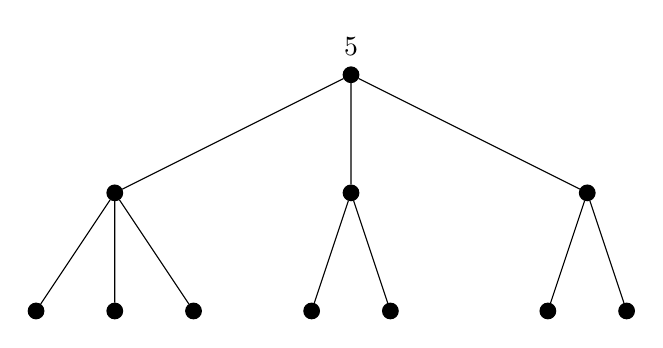
\begin{tikzpicture}[scale = 1,every node/.style={circle,draw, fill= black, inner sep = 2pt},level 1/.style={sibling 				distance=30mm},level 2/.style={sibling distance=10mm}]
	
	\node[label = above:5] {}
	child {
		node{} 
		child {
			node{}
		}			
		child {
			node{}
		}
		child {
			node{}
		}
	}
	child {
		node{} 
		child {
			node{}
		}			
		child {
			node{}
		}
	}
	child {
		node{} 
		child {
			node{}
		}			
		child {
			node{}
		}
	};	
	\end{tikzpicture}

	% 8 - 6
	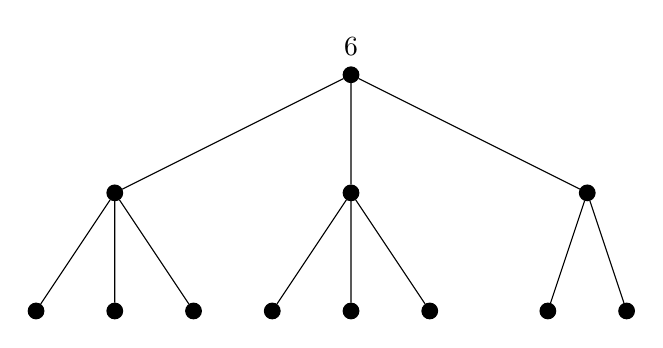
\begin{tikzpicture}[scale = 1,every node/.style={circle,draw, fill= black, inner sep = 2pt},level 1/.style={sibling 				distance=30mm},level 2/.style={sibling distance=10mm}]
	
	\node[label = above:6] {}
	child {
		node{} 
		child {
			node{}
		}			
		child {
			node{}
		}
		child {
			node{}
		}
	}
	child {
		node{} 
		child {
			node{}
		}			
		child {
			node{}
		}
		child {
			node{}
		}
	}
	child {
		node{} 
		child {
			node{}
		}			
		child {
			node{}
		}
	};	
	\end{tikzpicture}

	% 8 - 7
	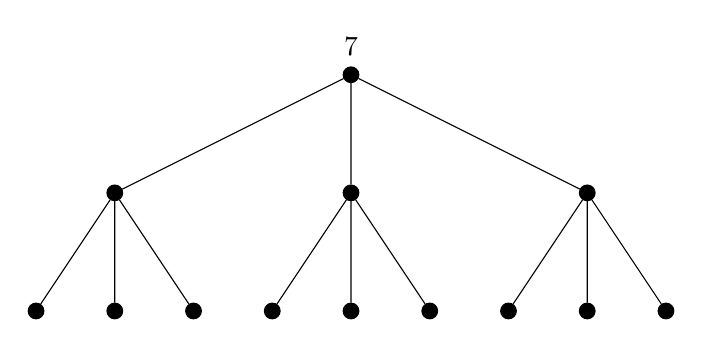
\begin{tikzpicture}[scale = 1,every node/.style={circle,draw, fill= black, inner sep = 2pt},level 1/.style={sibling 				distance=30mm},level 2/.style={sibling distance=10mm}]
	
	\node[label = above:7] {}
	child {
		node{} 
		child {
			node{}
		}			
		child {
			node{}
		}
		child {
			node{}
		}
	}
	child {
		node{} 
		child {
			node{}
		}			
		child {
			node{}
		}
		child {
			node{}
		}
	}
	child {
		node{} 
		child {
			node{}
		}			
		child {
			node{}
		}
		child {
			node{}
		}
	};	
	\end{tikzpicture}

% 10
\seti{9}
\item Consider a full binary tree $T$ of height $h$.
	\be
	% 10a
	\item How many leaves does $T$ have?\\
	A full binary tree has $2^h$ leaves.
	% 10b
	\item How many vertices does $T$ have?\\
	A full $m$-ary tree has $\frac{m^{h+1}-1}{m-1}$ vertices, so\\
	a full binary tree has $\frac{2^{h+1}-1}{2-1}=2^{h+1}-1$ vertices.
	\ee

% 12
\seti{11}
\item Give some real-life examples of information storage that can be viewed as labeled trees.\\
A labeled tree can be used to visualize a family tree, and a labeled tree can also be used to visualize the syntax of a language.

% Additional Problem 1
\seti{0}
\item Additional Problem: Draw a tree with Prufer code (5,2,1,4,4,1,6,1,1), with no crossing edges. Show some work.
	\begin{align*}
	(5,2,1,4,4,1,6,1,1) &\to& 
	(\not5,2,1,4,4,1,6,1,1) &\to& 
	\\
	\{1,2,3,4,5,6,7,8,9,10,11\} &\to& 
	\{1,2,\not3,4,5,6,7,8,9,10,11\} &\to& 
	\\
	\\
	(\not5,\not2,1,4,4,1,6,1,1) &\to&
	(\not5,\not2,\not1,4,4,1,6,1,1) &\to& 
	\\
	\{1,2,\not3,4,\not5,6,7,8,9,10,11\} &\to&
	\{1,\not2,\not3,4,\not5,6,7,8,9,10,11\} &\to& 
	\\
	\\
	(\not5,\not2,\not1,\not4,4,1,6,1,1) &\to& 
	(\not5,\not2,\not1,\not4,\not4,1,6,1,1) &\to&
	\\
	\{1,\not2,\not3,4,\not5,6,\not7,8,9,10,11\} &\to&
	\{1,\not2,\not3,4,\not5,6,\not7,\not8,9,10,11\} &\to&
	\\ 
	\\
	(\not5,\not2,\not1,\not4,\not4,\not1,6,1,1) &\to& 
	(\not5,\not2,\not1,\not4,\not4,\not1,\not6,1,1) &\to& 
	\\
	\{1,\not2,\not3,\not4,\not5,6,\not7,\not8,9,10,11\} &\to& 
	\{1,\not2,\not3,\not4,\not5,6,\not7,\not8,\not9,10,11\} &\to&
	\\
	\\
	(\not5,\not2,\not1,\not4,\not4,\not1,\not6,\not1,1) &\to&
	(\not5,\not2,\not1,\not4,\not4,\not1,\not6,\not1,\not1) &\to&
	\\
	\{1,\not2,\not3,\not4,\not5,\not6,\not7,\not8,\not9,10,11\} &\to&
	\{1,\not2,\not3,\not4,\not5,\not6,\not7,\not8,\not9,\not{10},11\} &\to&
	\\
	\\
	(\not5,\not2,\not1,\not4,\not4,\not1,\not6,\not1,\not1) &\to&
	\\
	\{\not1,\not2,\not3,\not4,\not5,\not6,\not7,\not8,\not9,\not{10},\not11\} &\to&
	\end{align*}
	\[
	\to\{(5,3),(2,5),(1,2),(4,7),(4,8),(1,4),(6,9),(1,6),(1,10),(1,11)\}
	\]
	
	\begin{tikzpicture}[scale = 1,every node/.style={circle,draw, fill= black, inner sep = 2pt},level 1/.style={sibling 				distance=30mm},level 2/.style={sibling distance=10mm}]
	
	\node[label = above:1] {}
	child {
		node[label = left:2]{} 
		child {
			node[label = left:5]{}
			child {
				node[label = right:3]{}
			}
		}
	}
	child {
		node[label = left:4]{} 
		child {
			node[label = left:7]{}
		}
		child {
			node[label = right:8]{}
		}
	}
	child {
		node[label = right:6]{} 
		child {
			node[label = right:9]{}
		}
	}
	child {
		node[label = right:10]{} 
	}
	child {
		node[label = right:11]{} 
	};	
	\end{tikzpicture}

\item Find the Pr\"{u}fer code of the following tree. Show some work.

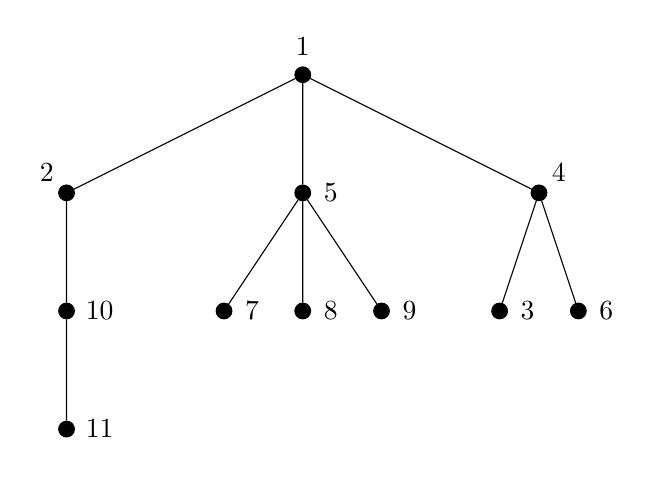
\begin{tikzpicture}[scale = 1,every node/.style={circle,draw, fill= black, inner sep = 2pt},level 1/.style={sibling distance=30mm},level 2/.style={sibling distance=10mm}
]
\node[label = above:1] {}
child { node[label = above left:2] {} child { node[label = right:10] {} child { node[label = right:11] {} }}}
child { node[label = right:5] {} 
child { node[label = right:7] {} }
child { node[label = right:8] {} }
child { node[label = right:9] {} }
}
child { node[label = above right:4] {} 
child { node[label = right:3] {} }
child { node[label = right:6] {} }};

\end{tikzpicture}
	\\
	\{Leaf (Neighbor),\} $\to$ \{3 (4), 6 (4), 4 (1), 7 (5), 8 (5), 9 (5), 5 (1), 1 (2), 2 (10)\} \\
	$\to\paren{4,4,1,5,5,5,1,2,10}$
	
\ee

% SECTION 6.5 # 2, 4, 8
\be

% 2
\seti{1}
\item For each graph, give a Hamilton circuit or explain why none exists.
	\be
	% 2a
	\item
	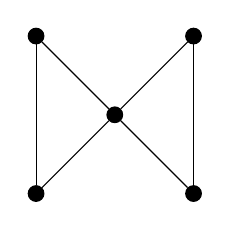
\begin{tikzpicture}
	\begin{scope}[every node/.style={circle,draw, fill= black, inner sep = 2pt}]
	    	\node (1) at (0,0) {};
		\node (2) at (0,2) {};
	    	\node (3) at (2,2) {};
		\node (4) at (2,0) {};
	    	\node (5) at (1,1) {};
	\end{scope}
	
	\begin{scope}[>={Stealth[black]},
	              every node/.style={fill=white,circle},
	              every edge/.style={draw=black}]
		\path (1) edge (2);
		\path (2) edge (5);
		\path (3) edge (5);
		\path (4) edge (5);
		\path (3) edge (4);
		\path (1) edge (5);
	\end{scope}
	\end{tikzpicture}
		\\
		A Hamilton circuit does not exist because the center vertex must always be passed twice in order to reach all the 
		vertices.
	% 2b
	\item 
	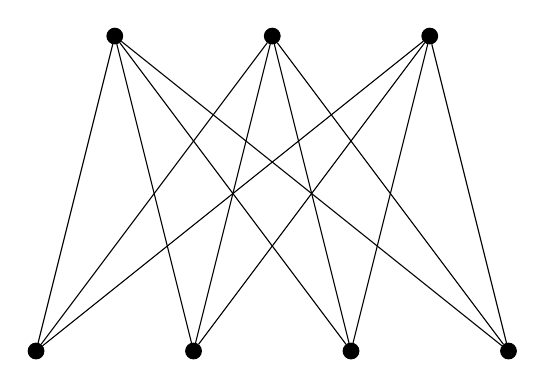
\begin{tikzpicture}
	\begin{scope}[every node/.style={circle,draw, fill= black, inner sep = 2pt}]
	    	\node (1) at (0,0) {};
		\node (2) at (2,0) {};
	    	\node (3) at (4,0) {};
		\node (4) at (6,0) {};
	    	\node (5) at (1,4) {};
		\node (6) at (3,4) {};
	    	\node (7) at (5,4) {};
	\end{scope}
	
	\begin{scope}[>={Stealth[black]},
	              every node/.style={fill=white,circle},
	              every edge/.style={draw=black}]
		\path (1) edge (5);
		\path (1) edge (6);
		\path (1) edge (7);
		\path (2) edge (5);
		\path (2) edge (6);
		\path (2) edge (7);
		\path (3) edge (5);
		\path (3) edge (6);
		\path (3) edge (7);
		\path (4) edge (5);
		\path (4) edge (6);
		\path (4) edge (7);
	\end{scope}
	\end{tikzpicture}
		\\
		Observe that the graph is bipartite because there exists 2 subsets $V_1\text{ and }V_2$ where every edge in the graph
		connects a vertex in $V_1$ to $V_2$. Suppose The vertices of $V_1$ are the top 3 and the vertices of $V_2$ are the 
		bottom 4:  $|V_1|=3$ and $|V_2|=4$. Notice that $|V_1|\not=|V_2|$ so there can't be a Hamilton circuit by Theorem 4.

	% 2c
	\item
	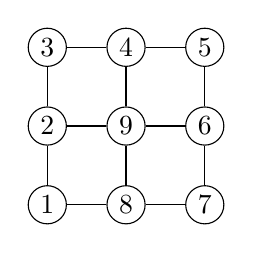
\begin{tikzpicture}
	\begin{scope}[every node/.style={circle,draw, inner sep = 2pt}]
	    	\node (1) at (0,0) {$1$};
		\node (2) at (0,1) {$2$};
	    	\node (3) at (0,2) {$3$};
		\node (4) at (1,2) {$4$};
	    	\node (5) at (2,2) {$5$};
		\node (6) at (2,1) {$6$};
	    	\node (7) at (2,0) {$7$};
		\node (8) at (1,0) {$8$};
	    	\node (9) at (1,1) {$9$};
	\end{scope}
	
	\begin{scope}[>={Stealth[black]},
	              every node/.style={fill=white,circle},
	              every edge/.style={draw=black}]
		\path (1) edge (2);
		\path (1) edge (8);
		\path (2) edge (3);
		\path (2) edge (9);
		\path (3) edge (4);
		\path (4) edge (5);
		\path (4) edge (9);
		\path (5) edge (6);
		\path (6) edge (7);
		\path (6) edge (9);
		\path (7) edge (8);
		\path (8) edge (9);
	\end{scope}
	\end{tikzpicture}
		\\
		Observe that the graph is bipartite by splitting the the graph into subgraphs\\
		$V_1=\{1,3,5,7,9\}\text{ and }V_2=\{2,4,6,8\}$. Notice that $|V_1|=5\text{ and }|V_2|=4$. \\
		$|V_1|\not=|V_2|$ so by Theorem 4 there can't be a Hamilton circuit.
	
	\ee














\ee

\end{document}